\section{eo\-One\-Fifth\-Mutation$<$ EOT $>$ Class Template Reference}
\label{classeo_one_fifth_mutation}\index{eoOneFifthMutation@{eoOneFifthMutation}}
the dynamic version: just say it is updatable - and write the {\bf update()}{\rm (p.\,\pageref{classeo_one_fifth_mutation_a3})} method! here the 1 fifth rule: count the proportion of successful mutations, and increase sigma if more than threshold (1/5 !)  


{\tt \#include $<$eo\-Normal\-Mutation.h$>$}

Inheritance diagram for eo\-One\-Fifth\-Mutation$<$ EOT $>$::\begin{figure}[H]
\begin{center}
\leavevmode
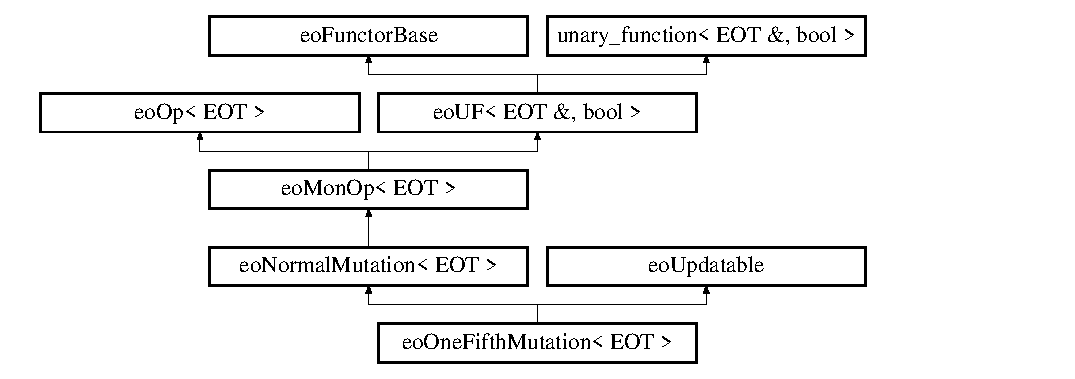
\includegraphics[height=4.64345cm]{classeo_one_fifth_mutation}
\end{center}
\end{figure}
\subsection*{Public Types}
\begin{CompactItemize}
\item 
typedef EOT::Fitness {\bf Fitness}\label{classeo_one_fifth_mutation_w0}

\end{CompactItemize}
\subsection*{Public Member Functions}
\begin{CompactItemize}
\item 
{\bf eo\-One\-Fifth\-Mutation} ({\bf eo\-Eval\-Func}$<$ {\bf EOT} $>$ \&\_\-eval, double \&\_\-sigma\-Init, unsigned \_\-window\-Size=10, double \_\-update\-Factor=0.83, double \_\-threshold=0.2)
\begin{CompactList}\small\item\em (Default) Constructor. \item\end{CompactList}\item 
virtual std::string {\bf class\-Name} () const \label{classeo_one_fifth_mutation_a1}

\begin{CompactList}\small\item\em The class name. \item\end{CompactList}\item 
bool {\bf operator()} ({\bf EOT} \&\_\-eo)
\begin{CompactList}\small\item\em Do it! calls the standard mutation, then checks for success and updates stats. \item\end{CompactList}\item 
void {\bf update} ()\label{classeo_one_fifth_mutation_a3}

\begin{CompactList}\small\item\em the method that will be called every generation if the object is added to the checkpoint \item\end{CompactList}\end{CompactItemize}
\subsection*{Private Attributes}
\begin{CompactItemize}
\item 
{\bf eo\-Eval\-Func}$<$ {\bf EOT} $>$ \& {\bf eval}\label{classeo_one_fifth_mutation_r0}

\item 
double {\bf threshold}\label{classeo_one_fifth_mutation_r1}

\item 
double {\bf update\-Factor}\label{classeo_one_fifth_mutation_r2}

\item 
std::vector$<$ unsigned $>$ {\bf nb\-Mut}\label{classeo_one_fifth_mutation_r3}

\item 
std::vector$<$ unsigned $>$ {\bf nb\-Success}\label{classeo_one_fifth_mutation_r4}

\item 
unsigned {\bf gen\-Index}\label{classeo_one_fifth_mutation_r5}

\end{CompactItemize}


\subsection{Detailed Description}
\subsubsection*{template$<$class EOT$>$ class eo\-One\-Fifth\-Mutation$<$ EOT $>$}

the dynamic version: just say it is updatable - and write the {\bf update()}{\rm (p.\,\pageref{classeo_one_fifth_mutation_a3})} method! here the 1 fifth rule: count the proportion of successful mutations, and increase sigma if more than threshold (1/5 !) 



Definition at line 177 of file eo\-Normal\-Mutation.h.

\subsection{Constructor \& Destructor Documentation}
\index{eoOneFifthMutation@{eo\-One\-Fifth\-Mutation}!eoOneFifthMutation@{eoOneFifthMutation}}
\index{eoOneFifthMutation@{eoOneFifthMutation}!eoOneFifthMutation@{eo\-One\-Fifth\-Mutation}}
\subsubsection{\setlength{\rightskip}{0pt plus 5cm}template$<$class EOT$>$ {\bf eo\-One\-Fifth\-Mutation}$<$ {\bf EOT} $>$::{\bf eo\-One\-Fifth\-Mutation} ({\bf eo\-Eval\-Func}$<$ {\bf EOT} $>$ \& {\em \_\-eval}, double \& {\em \_\-sigma\-Init}, unsigned {\em \_\-window\-Size} = {\tt 10}, double {\em \_\-update\-Factor} = {\tt 0.83}, double {\em \_\-threshold} = {\tt 0.2})\hspace{0.3cm}{\tt  [inline]}}\label{classeo_one_fifth_mutation_a0}


(Default) Constructor. 

\begin{Desc}
\item[Parameters:]
\begin{description}
\item[{\em eval}]the evaluation function, needed to recompute the fitmess \item[{\em \_\-sigma\-Init}]the initial value for uniform mutation \item[{\em \_\-window\-Size}]the size of the window for statistics \item[{\em \_\-threshold}]the threshold (the 1/5 - 0.2) \item[{\em \_\-update\-Factor}]multiplicative update factor for sigma \end{description}
\end{Desc}


Definition at line 195 of file eo\-Normal\-Mutation.h.

\subsection{Member Function Documentation}
\index{eoOneFifthMutation@{eo\-One\-Fifth\-Mutation}!operator()@{operator()}}
\index{operator()@{operator()}!eoOneFifthMutation@{eo\-One\-Fifth\-Mutation}}
\subsubsection{\setlength{\rightskip}{0pt plus 5cm}template$<$class EOT$>$ bool {\bf eo\-One\-Fifth\-Mutation}$<$ {\bf EOT} $>$::operator() ({\bf EOT} \& {\em \_\-eo})\hspace{0.3cm}{\tt  [inline, virtual]}}\label{classeo_one_fifth_mutation_a2}


Do it! calls the standard mutation, then checks for success and updates stats. 

\begin{Desc}
\item[Parameters:]
\begin{description}
\item[{\em \_\-eo}]The chromosome undergoing the mutation \end{description}
\end{Desc}


Reimplemented from {\bf eo\-Normal\-Mutation$<$ EOT $>$} {\rm (p.\,\pageref{classeo_normal_mutation_a3})}.

Definition at line 216 of file eo\-Normal\-Mutation.h.

References EO$<$ F $>$::fitness(), EO$<$ F $>$::invalid(), EO$<$ F $>$::invalidate(), and eo\-Normal\-Mutation$<$ EOT $>$::operator()().

The documentation for this class was generated from the following file:\begin{CompactItemize}
\item 
eo\-Normal\-Mutation.h\end{CompactItemize}
